\documentclass[titlepage]{article}
\usepackage[labelfont=bf]{caption}
\usepackage{float}
\usepackage{caption}
\usepackage{wrapfig}
\usepackage{geometry}
\usepackage{graphicx}
\usepackage{multirow}
\usepackage{adjustbox}
\usepackage{textcomp}
\usepackage{courier}
\usepackage{setspace}
\captionsetup*[subfigure]{position=bottom}
\setlength\headheight{1pt}

\begin{document}
\begin{center}
\vspace*{\fill}
\LARGE{\textbf{BME 261: Detecting Freezing of Gait in Parkinson's Patients}}
\vspace{1cm}

\Large{Laura Ing\linebreak Charly Phillips\linebreak Daphne Walford\linebreak Zhiling (Zoe) Zou\linebreak Arrchana Pradeepan \linebreak\linebreak December 5, 2016}
\end{center}
\vspace*{\fill}
\clearpage

\tableofcontents

\begin{doublespacing}

\clearpage
\section{Executive Summary}
\subsection{Design aspects}

The purposes of this project are to (1) successfully detect freezing of gait (FOG) experienced by Parkinson's patients, using signals from an inertial measurement unit (IMU), and (2) to activate a motor and buzzer upon FOG onset. The device designed to meet these goals is called AntiFreeze, and consists of two major components: a physical prototype, and a FOG detection algorithm. 

The physical prototype houses a circuit incorporating an Arduino microcontroller, which powers an IMU, a motor, and a buzzer. The IMU is able to detect linear and angular acceleration with an accelerometer and gyroscope, respectively, and is used for collecting data pertaining to a person's gait so that it may be analysed. Once the algorithm has detected freezing, an LED blinks, the buzzer sounds and the motor runs, providing mechanical stimulation to the Achilles tendon. The Arduino and IMU are attached to the person's foot while a pouch holding the remaining hardware components is strapped to the calf. This pouch holds the buzzer, motor, battery, and second breadboard, which are secured with Velcro inside the pouch. Wires protected by a plastic tube run between the two breadboards along the length of the calf. 

The second component of the design involves the FOG detection algorithm. First, IMU signals are read into the Arduino, specifically gyroscope Y values. Next, a novel smoothing algorithm is applied to the signal, removing noise to distinguish freezing signals from walking and stopping signals. Smoothed data is then processed to identify the periods and amplitudes of every waveform in the signal. Periods and amplitudes within set threshold values are detected as freezing and trigger the onset of the motor, buzzer and LED. 

\subsection{Performance}

Given that the requirements for AntiFreeze were to process the gait signals of Parkinson's patients and activate a stimulus on detecting FOG, the device performed above expectations. It was able to meet these requirements consistently without fail, including difficult cases such as turning and walking up and down stairs. The device met not only the requirement of turning on a motor upon detection of FOG, but also activated a buzzer and LED. To house all the various hardware components together, a denim pouch was designed to hold the motor's axle against the Achilles tendon, and loose wires were housed in attached tubing to ensure compactness. Though the positioning of the IMU (horizontally placed on the top of the foot) resulted in a lot of low amplitude noise in the signal, the filtering algorithm eliminated this issue, as seen by the accurate onset of stimulus output. On the whole, the current prototype for AntiFreeze exceeded expectations. 

\subsection{Improvements}

Although the device's current performance is more than satisfactory, several improvements could be made to future redesigns. On the side of software signal detection, refactoring methods could be further applied to existing code to ensure efficiency, readability, and easy editing. Additionally, statistical calculations such as t-tests and confidence intervals could be integrated into a calibration step to help establish accurate threshold values, which would enable various individuals to be able to use one device, rather than hardcoding in threshold values specific to one individual. The device's physical design could be improved by making it sleeker, thus enclosing all the hardware components into one sleeve that can slide over the calf. As well, to further ensure user comfort, a hardware design that incorporates fewer, smaller and lighter hardware components can be looked into. Replacing both breadboards with a customized and flexible PCB that sits more comfortably on the back of the calf would be an excellent eventual option.

\clearpage
\section{Background}

Parkinson's disease is an increasingly common neurological disorder which poses severe impairments to both the motor and cognitive functioning of patients. One of its most debilitating symptoms is freezing of gait, as it limits independence, causes frustration, and increases the risk of falling. Freezing of gait is typically triggered by walking through narrow spaces, such as doorways, or by turning. It is characterised by rapid flexing of the foot (in an attempt to walk), as well as shaking and shuffling of the feet. As such, there is a need for a device able to detect freezing of gait and apply stimulation in the form of vibration in order to counteract the freezing. 

Vibration in the Achilles tendon has been shown to reduce movement errors in patients with Parkinson's disease \cite{almeida}. The stimulus should therefore be applied against the back of the patient's ankle, near the heel. In order to detect freezing, an accelerometer and gyroscope sensor will need to be placed in a location appropriate for detecting fluctuations in the subject's motion, but without sacrificing the comfort of the patient or further compromising their ability to walk. By extension, the design will need to be fairly compact so that wires and other components do not become tripping hazards, as well as relatively lightweight to minimize muscle fatigue during walking. Most importantly, the device will need to be able to differentiate freezing from walking and stopping, and thus must be able to identify common trends during these three different gait signal phases. Furthermore, it should indicate when freezing has occurred in the most salient way possible, perhaps through both visual and auditory cues. Lastly, the physical design should be adjustable for patients of varying anatomies.

\clearpage
\section{Design and Prototype}
\subsection{Physical design}

\begin{figure}[H]
	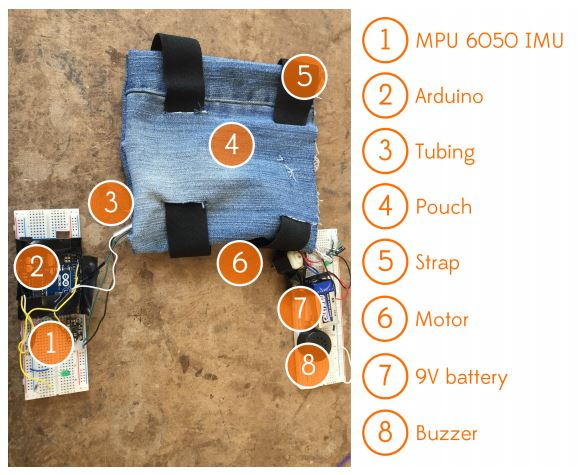
\includegraphics[width=\linewidth]{labelled-design}
	\caption{Labelled diagram of the physical prototype.}
	\label{labelled}
\end{figure}

The physical design of AntiFreeze has two main components. The first component includes the breadboard found on top of the patient's shoe, which houses the IMU and Arduino (as depicted in Figure \ref{labelled} by 1 and 2). The first necessary design decision was where the IMU should be placed. The two options the team debated were placing the IMU horizontally on the top of the foot, or vertically on the back of the calf. It was decided that the IMU should be placed on the top of the foot, because the signal of interest was Gyroscope-Y and this positioning allowed for the greatest sensitivity in the change in units from the horizontal. The second design decision that needed to be made was how to house hardware that needed to sit over the Achilles tendon, including the placement of the motor, buzzer, and their associated required hardware components. In accordance with available resources, a denim pouch was designed to encompass these components. This design is visible in Figure \ref{on-foot} below, and incorporates straps (shown as 4 and 5 in Figure \ref{labelled}), which hold in place a second breadboard that contains the motor, battery, and buzzer (denoted by 6, 7, and 8 in Figure \ref{labelled}). The denim material was chosen due to its familiarity among users. The incorporation of the straps allow the sleeve to be adjustable to different leg sizes and anatomies.

\begin{wrapfigure}[13]{l}{6.5cm}
	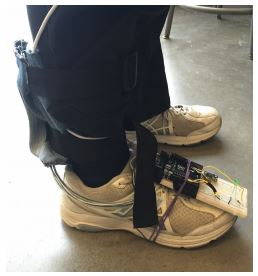
\includegraphics[width=\linewidth]{on-foot}
	\caption{Prototype set up on person.}
	\label{on-foot}
\end{wrapfigure}

Since the motor provides the stimulus necessary to counteract freezing, its axle protrudes from a slit in the back of the sleeve, so that there is direct contact between it and the Achilles tendon. The buzzer was incorporated into the design to provide an auditory warning to the caregiver that their patient is at risk of falling. Although a smaller buzzer was originally taped to the outside of the pouch to make its signal more audible, there was too much strain on its lead wires, which resulted in their eventual breakage. As a result, a louder and more durable buzzer (labelled 8 in Figure \ref{labelled}) was incorporated into the breadboard inside the pouch. Wires needed to provide a connection between the hardware in the pouch and the Arduino pass through a compact and flexible plastic tube (component 3 in Figure \ref{labelled}), allowing pouch components to receive required signals from the Arduino.

\begin{figure}[H]
	\centering
\begin{minipage}{.9\textwidth}
	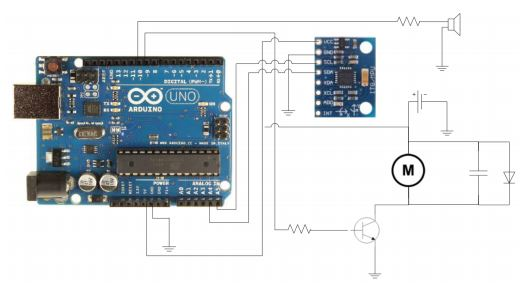
\includegraphics[width=\linewidth]{arduino}
	\caption{Circuit schematic.}
	\label{arduino}
\end{minipage}
\end{figure}

Figure \ref{arduino}, above, shows the schematic of our circuit. The Arduino controls the buzzer and motor/transistor from pins 10 and 9 respectively, as they have pulse width modulation capabilities. The motor system is the most complicated part of the circuit, as it consists of a DC motor, transistor, capacitor, LED, and battery. The 9V battery powers the motor directly so that it does not draw power from the Arduino, which could potentially exceed the maximum amount of voltage it can provide. The transistor controls the motor electrically by determining the amount of voltage the collector receives and therefore the amount the emitter provides. The LED prevents a large voltage drop in the circuit when the motor is turned off, and the capacitor reduces the amount of noise in the circuit. Although the onboard LED, controlled by pin 13, was originally used, it was later decided to use an external LED, controlled by pin 12, which produced clearer visual signals. This is not shown in the schematic. The IMU has pins running to 5V and ground as well as the clock and data lines, which correlate to pins A5 and A4. This is required to be able to read signals for the software detection of freezing. To power the Arduino without a computer, we used a compact external battery pack that would be much easier for patients to recharge when required. This design decision was an obvious choice over having a laptop constantly connected to the Arduino in order to power it.

\subsection{Software design}

On the side of signal processing, the signal chosen was the value outputted by the IMU for Gyroscope-Y. This signal was selected due to its distinct features, which were a result of the placement of the IMU. Gyroscope-Y measures angular change per second in the y-direction, and as mentioned above, because the IMU was placed horizontally on the top of the foot, the raising and lowering of the foot was easily picked up in this signal. In fact, this is visible in Figure \ref{graphs} below; the orange signal on the second subplot represents Gyroscope-Y. The signal consists of very distinct values for period and amplitude for each step taken during walking, freezing and stopping, and that is why the amplitude and period of one step cycle were chosen for freezing detection. It was observed that during walking, amplitude and period were at a maximum, whereas during stopping these features were at a minimum of approximately near zero. During freezing, these features were consistently found to be at an intermediate period and amplitude between the maximum and minimum. By implementing a dual-feature-check that ensures both the amplitude and period are between a threshold, FOG signals were easily detected.

\begin{figure}[H]
	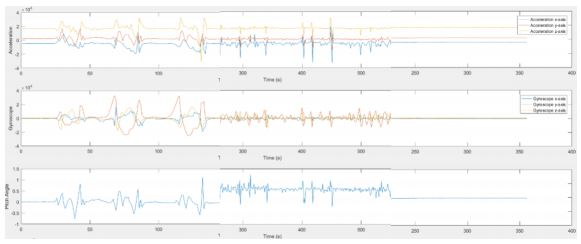
\includegraphics[width=\linewidth]{graphs}
	\caption{IMU acceleration, gyroscope and pitch angle values plotted against time for walking, freezing and stopping (Disclaimer: this figure contains 9 plots with walking, freezing and stopping signals placed next to each other for easy comparison. As a result, the labelled time axis values may not be accurate).}
	\label{graphs}
\end{figure}

In terms of the design of the signal filter, the Gyroscope-Y signal was filtered using a novel algorithm that zeroed consecutive Gyroscope-Y values with a difference of less than 20 units. This made FOG detection much easier, as noise between steps and during walking were leveled to a value of zero. 

Below is a code excerpt, from the filtration step.

\newenvironment{code}{\ttfamily}{\par}
\begin{code}
\noindent long filter(long Gy) { \\
\indent  if (abs(Gy - prevGy)< 20) return prevGy; // small fluctuation \\
  return Gy; \\
}
\end{code}

Stimuli were activated when both the amplitude and period were found to be within a threshold indicative of freezing. However, to ensure that freezing and freezing-like-motion could be differentiated, a counter was implemented, as this ensured that a minimal amount of freezing-like-motion was detected before turning on the stimuli.

    In terms of alternatives for signal choice, any other signal found in Figure \ref{graphs} could have been selected for the purpose of this project. However, the hardcoded threshold values used to detect FOG would have to be set to reflect the new signal, which may prove difficult given that the difference in amplitude and period between walking and freezing is not as obvious for the other IMU signals. Thus, if an alternative signal were to be utilized, new features might need to be identified in order to detect freezing. Due to this, a more powerful filtration method might also be required, as the differences in amplitude and period between different gait signal phases are not as pronounced in signals other than Gyroscope-Y.

\clearpage
\section{Results}

Upon implementation of the filtration step, the Gyroscope-Y signal found in Figure \ref{graphs}, above, was filtered to look like the signal found in Figure \ref{filtered}, below. If Figure \ref{filtered} is analyzed carefully, it can be seen that in the periods of time between each step, almost no noise in the signal exists, as denoted by the straight lines. This made the measurement of period and amplitude easy, as change was easily detectable. Amplitude measurements less than 300 units and period measurements less than 0.6 units incremented a counter. When this counter reaches 3, output stimuli devices are switched on, as significant freezing is detected at this point.

\begin{figure}[H]
	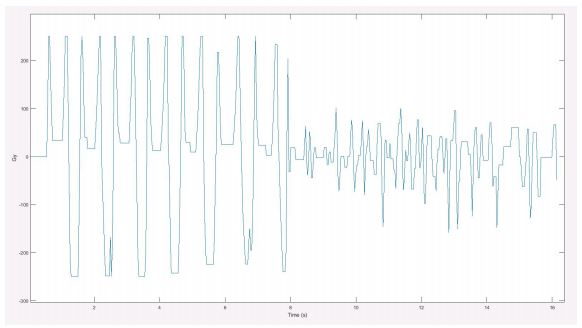
\includegraphics[width=\linewidth]{filtered}
	\caption{Filter walking and freezing Gyroscope-Y signals}
	\label{filtered}
\end{figure}

Figure \ref{serial} provides an example snippet of what was output to the Arduino serial monitor for the above signal around the transition between walking and freezing. As you can see, for every step taken, or fluctuation in signal, values for amplitude and period are calculated and outputted. If the amplitude or period is greater than the established threshold values, the counter is incremented. Once the counter reaches 3, freezing is detected, as identified by the “freezing” message in the output.

\begin{figure}[H]
	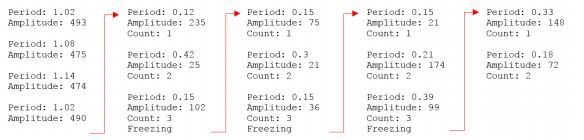
\includegraphics[width=\linewidth]{serial}
	\caption{Arduino serial monitor output for the signal found in Figure \ref{filtered}, specifically at the transition of walking to freezing}
	\label{serial}
\end{figure}

The robustness of our filtration and signal detection is clearly seen in Figure \ref{w-f-period} below. There is a distinct separation in period values for non-freezing (blue) and freezing (red). In fact, to further prove the connection between Figure \ref{filtered} and Figure \ref{w-f-period}, the initial seven obvious fluctuations in signal seen in Figure \ref{filtered} are represented by the seven blue period markers indicated in the plot below.

\begin{figure}[H]
\centering
\begin{minipage}{.45\textwidth}
	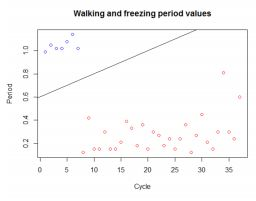
\includegraphics[width=\linewidth]{w-f-period}
	\caption{Period values plotted against cycle, which is the index associated with each step taken, for the signal found in Figure 4}
	\label{w-f-period}
\end{minipage}\hfill
\begin{minipage}{.45\textwidth}
	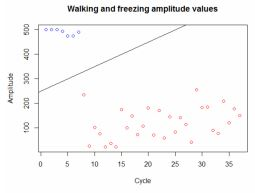
\includegraphics[width=\linewidth]{w-f-amplitude}
	\caption{Amplitude values plotted against cycle, which is the index associated with each step taken, for the signal found in Figure 4}
	\label{w-f-amplitude}
\end{minipage}
\end{figure}

Similarly, calculated amplitude values exhibited an equally strong distinction between freezing and non-freezing for every step taken to produce the signal in Figure \ref{filtered}. Thus, overall it seems fair to conclude that the features and thresholds used to detect freezing are correct and robust.

\clearpage
\section{Analysis}
\subsection{Physical design}
Although several design decision turned out very well, improvements could be made for future iterations. The integration of three output devices--the motor, LED and buzzer--provided important functionality to the primary and secondary users of the device. Caregivers are notified during FOG, and the patient's muscle is stimulated. These design elements are definitely something to maintain for future iterations.

Likewise, the decision to place the MPU 6050 IMU on the top of the foot was on the whole a good choice. For one, it was an optimal position to read Gyroscope-Y values since the IMU was parallel to the horizontal ground. In addition, the difference between freezing and normal walking was more conspicuous in the signals produced, as its direct contact with the foot made it extremely sensitive to rapid flexing of the foot, a trademark of freezing. 

However, as a result of this decision, a series of design decisions were made that affected the compactness and simplicity of the design. To begin with, a breadboard housing the IMU and Arduino was placed on the foot, which was somewhat awkward and tended to interfere with walking. The effect was particularly pronounced when the patient wore lace-up shoes with a prominent tongue, similar to the orthotic shoes frequently favoured by the elderly, as this caused the breadboard to slip down the foot. Bulky objects, such as the breadboard strapped to the foot, would also be especially inconvenient for the main demographic of Parkinson's disease patients, who are senior citizens and may already have other health issues which hinder walking, such as arthritis. Furthermore, the placement of the breadboard on the foot resulted in the incorporation of a second breadboard to hold the motor, buzzer, and battery in the pouch, against the Achilles tendon. This resulted in a need for a connective tube to hold wires running between the two breadboards. Ultimately, the placement of hardware components in multiple different areas resulted in a design that was bulky, complicated and put patients at risk of tripping.

\subsection{Software design}

After extensive testing and modifications were conducted on the threshold values numerous times, the software based FOG detection consistently activated stimuli during FOG only. The software was not only proven to work with regular cases of walking, freezing and stopping, but unique cases were also tested to further determine the performance of the device. For example, FOG stimuli were not switched on while walking down stairs, turning at various angles, or during other common motions. This accuracy is largely due to the choice of signal (Gyroscope-Y), as its features fluctuate dramatically during change in vertical motion. The filtration component also lends a hand in eliminating noise in the signal that could be miscalculated to be freezing. 

A major shortcoming of the design, however, is the hardcoded threshold values for amplitude and period. This is due to the fact that different users have distinct differences in their physical structures,  which results in different gait patterns. Due to this, every time a new user is interested in using the device, IMU sample data during walking, freezing and stopping must be collected from the patient. Statistical analysis must then be performed to determine a distinct threshold value. Thresholds must then be hardcoded into the Arduino FOG detection algorithm. Overall, the accuracy of FOG detection is reduced when the device is shared between multiple users, as threshold values for amplitude and period are likely to vary between users of different walking styles and body types.

\clearpage
\section{Redesign Recommendations}

Although this device exceeds the requirements set out for it, multiple modifications could greatly improve its performance. The first changes relate to the algorithmic component of the device. Software refactoring involves encapsulating code into individual functions, allowing a program to be easily understood: instead of trying to figure out what blocks of code do, the reader parses through various clearly-named function calls. This practice promotes not only legibility but also easy editing, since sections of code are separated and can be tested and modified independently. This process could be applied in more depth to the current algorithm, since it has multiple function calls which would benefit from breakup and reorganisation.
Additionally, the threshold values used to detect freezing are currently hardcoded. They perform very consistently for the current subject, but Parkinson's disease affects an expansive age demographic--from those under 50 to individuals well over 90. Patients' walk cycles will therefore vary a great deal and the current threshold values may fail in some cases. A calibration script could run before the freezing detection period, while the subject attempts to walk a few steps, in order to collect information on the subject's motion patterns and then calculate threshold values for period and amplitude. The threshold values could be further ascertained through the use of statistical testing. If a t-test gives a poor result, indicating that the threshold value is potentially inaccurate and may have been calculated from irregular data, the calibration step could be programmed to repeat.

    As the device is currently powered by two batteries, an external battery pack and a 9V, it would be better to have the whole circuit powered by only one source so that the user could change the battery easily and from only one location. It would also be useful for the patient to know when this battery needed to be changed. This could be done by adding a multicolour LED to the circuit which changes colour between red, yellow, and green depending on the remaining voltage level. The voltage could be measured using a voltage divider with large resistor values so that the amount of voltage used by the divider were minimal. AnalogRead could be applied to detect when the voltage dropped below a certain level and the LED set to yellow. When the battery came close to draining, the LED would turn to red and the device would cease to function, forcing the patient to change the battery. 

A physical improvement could be made to improve the ease at which the two components can be put on. Currently the portion of the device that is placed on the calf is fairly easy to don and doff. However, the circuit on the foot is not. It would be easier if the Arduino were placed in the pouch and only the IMU remained on the foot. If the IMU was embedded into something similar to a sock with wires and a small circuit board running through/implanted in it, then it would be easier to put on.
Another hardware-related improvement to the design would be to program the buzzer to produce different pitches, or different rhythmic patterns, depending on how severe the freezing is. Patients often recover from an episode of freezing by themselves, and therefore do not require assistance from a caregiver \cite{pelosin}. However, sometimes this does not occur and the patient is at risk of falling if they are not assisted. Situation-dependent buzzer tones would provide the caregiver with a better idea of what kind of assistance the patient may need. For example, different auditory signals could correspond to slight shuffling (a slight increase in amplitude), high frequency shaking (large increase in amplitude), and stopping after a period of freezing, as the latter may mean the patient is about to fall. In addition, a different sound could be produced when the freezing occurs for a certain amount of time, as this would also indicate a high risk of falling.

     For future iterations, it is important to consider a more compact design for the AntiFreeze. The current denim pouch is convenient for storage of various device components, but it becomes more and more of a load on the calf as more and more components are added to it. A sleeker, compressed, sleeve like design containing a flexible PCB capable of sitting flush on the back of the calf should be looked into. The various hardware components currently found on both PCBs should also be connected to this one flexible PCB, and a circuit design of lighter and fewer components should be looked into. This would eliminate the current double loading placed on the foot and calf of the users, allowing for more comfortable wear. Additionally, having one single PCB house all the various components gets rid of the inconvenience associated with debugging the circuit in a situation where a component fails, falls out of place, or needs to be replaced. At a hardware component level, the integration of a louder buzzer would also be more helpful for caregivers of patients. 

\clearpage
\begin{thebibliography}{99}
\bibitem{almeida}
Tan, T.; Almeida, Q. J.; Rahimi, F.
(2011).
Proprioceptive deficits in Parkinson's disease patients with freezing of gait.
Neuroscience, Volume 192, Pages 746–752.

\bibitem{pelosin}
Pelosin et al.
(2010).
Action observation improves freezing of gait in patients with Parkinson's disease.
Neurorehabilitation and Neural Repair, XX(X) 1–7.

\end{thebibliography}
\end{doublespacing}
\end{document}